\documentclass[]{article}

\usepackage{amsmath}
\usepackage{amsfonts}
\usepackage{amssymb}

\usepackage[T1]{fontenc}
\usepackage{graphicx}
\usepackage{float}

\graphicspath{{./graphs/}}

%opening
\title{{{\normalsize Sprawozdanie drugie} \\
		{\huge Złożone struktury danych}}}
\author{Piotr Tylczyński}
\date{29.03.2019}

\begin{document}

\maketitle
\pagebreak

\section{Opisy}
	\subsection{Lista}
		Lista jest abstrakcyjnym typem danych. Dostęp do elemntów listy jest sekwencyjny, co oznacza, że odczytanie $ n. $ elemntu z listy, będzie wymagało odczytania $ n-1 $ pierwszych elemntów listy, co niekorzystnie wpływa na złożoność wielu algorytmów operujących na listach.
	\subsection{Drzewo AVL}
		Jego nazwa pochodzi od dwóch nazisk Adelsona-Velsky'ego i Landia, którzy byli jego twórcami. Jest to abstrakcyjna struktura danych, która jest samo balansującym się drzewem binarnym. Oznacza to, że jeśli która kolwiek z podgałęzi dowlonego węzła takiej struktury jest dłóższa od drugiej, nastepuje balansowanie drzewa. Taka właściwość pozytywnie wpływa na złożoność obliczeniową operacji przeszukiwania wspomnianej struktury.

\pagebreak
		
\section{Złożoność czasowa}
	\subsection{Szukanie elementu}
		\subsubsection{Lista}
			Algorytm szuukania elementu w liście szukając danego elementu musi przejżeć wszystkie elementu znajdujące się w liście aż do momentu kiedy nie trafi na szukany element. Powoduje to, że złożoność takiego algorytmu opisujemy przez:
			\[
				O(n) = n
			\]
		\subsubsection{Drzewo AVL}
			Jako, że drzewo AVL jest drzewem binarnym, to lewe dziecko dowolnego węzła w strukturze jset zawsze mnijsze od rodzica, a prawe większe. Taka zależność pozwala na każdorazowe odrzucenie połowy pozostałego do przeszukania zbioru, ponieważ wiadomo, że szukany element tam nie wystąpi. W związku z tym złożoność takiej operacji można określić jako:
			\[
			O(n) = \log_2{n}
			\]
			
	\subsection{Dodawanie n elementów w sposób posortowany}
		\begin{figure}[H]
			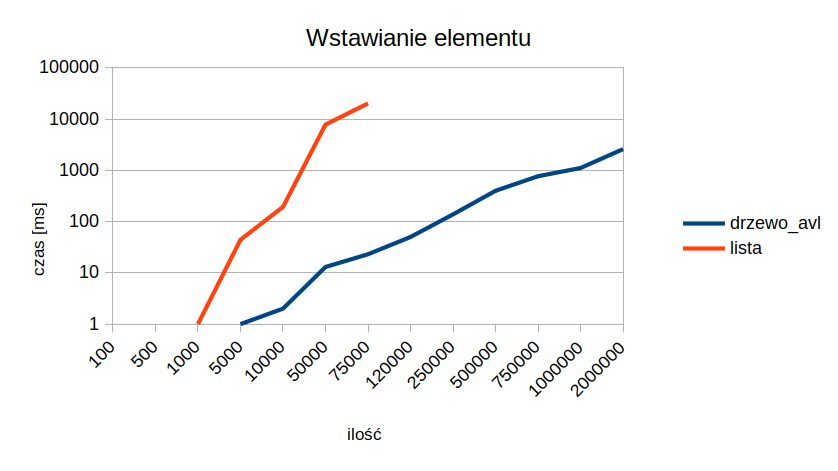
\includegraphics{insert.png}
		\end{figure}
		\subsubsection{Lista}
			Jak łatwo zauważyć czas wykonania rośnie bardzo szybko co jest spowodowane potrzebą przejżenia $ n-1 $ elemntów przed możliwością wstawienia nowego elementu $ n $. Dlatego w najgorszym przypadku - kiedy wartości elemntów są ułozone w kolejności odwrotnej do typu posortowania - algorytm wstawiania za każdym razem będzie musiał wyonać $n-1$ sprawdzeń, gdzie $n$ jest aktualną liczbą elemntów. Ogólnie złożonośc można przedstawić jako:
			\begin{multline}
			\text{ilość operacji} = (n-1) + (n-2) + (n-3) + ... + (n-n)  \\
			= n^2 + ...
			\end{multline}
			co daje złożoność:
			\[
			O(n) = n^2
			\]
		\subsubsection{Drzewo AVl}
			Ze względu na to, że drzewo AVL jest drzewam binarnym, jego wysokośc można opisać za pomocą logarytmu o podstawie 2. Oznacza to, że dodanie nowego elementu nie zajmie więcej operacji niż wysokość takiego drzewa. Dodatkowo drzewo po dodaniu elemntu należy zbalansować. Balansowanie zostaje zakończone w momencie znalezienia pierwsego nie zbalansowanego węzła. Złożoność wstawiania nowego elemntu opisujemy jako:
			\begin{equation}
				\begin{gathered}
				\text{ilość operacji} = k*(\text{szukanie miejsca} + \text{równoważenie}) \\
				
				\text{ilość operacji} = k*(\log\limits_{2}{n} + \log\limits_{2}{n}) \\
				
				O(n) = klog_2{n}
				\end{gathered}
			\end{equation}
			
		\subsection{Usuwanie losowych k elementów}
			\begin{figure}[H]
				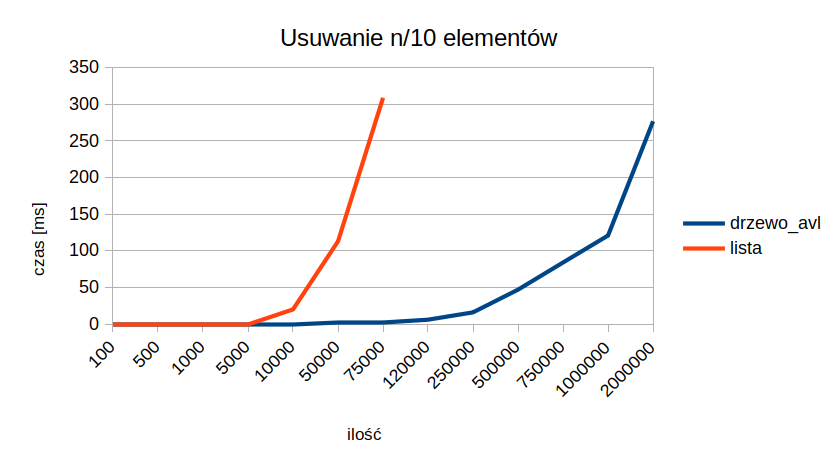
\includegraphics{remove.png}
			\end{figure}
			\subsubsection{Lista}
				Dostęp do $h$ elemntu wymaga sprawdzenia $h-1$ elementów. Wynika z tego, że złożoność wynosi
				\begin{equation}
					\begin{gathered}
						\text{ilość operacji} = k * \text{znalezienie elementu} \\
						
						O(n) = kn
					\end{gathered}
				\end{equation}

			\subsubsection{Drzewo AVL}
				Polega na znalezieniu usuwanego elementu w drzewie i wykonania algorytmu usuwania, w wyniku którego może zostać uruchomiony algorytm balansowania. Algorytm balansowania, nie kończy się w momencie znalezienia pierwszego niezbalansowanego węzła, jak w przypdaku dodawania elementu, lecz trwa do momentu kiedy całe drzewo nie zostanie ponowniezbalansowane.
				\begin{equation}
					\begin{gathered}
					\text{ilość operacji} = n * (\text{szukanie elementu} + \text{równoważenie}) \\
					
					\text{ilość operacji} = n * (\log\limits_{2}{n} + \log\limits_{2}{n}) \\
					
					O(n) = nlog_2{n}
					\end{gathered}
				\end{equation}
		\subsection{Usuwanie całej struktury}
			\begin{figure}[H]
				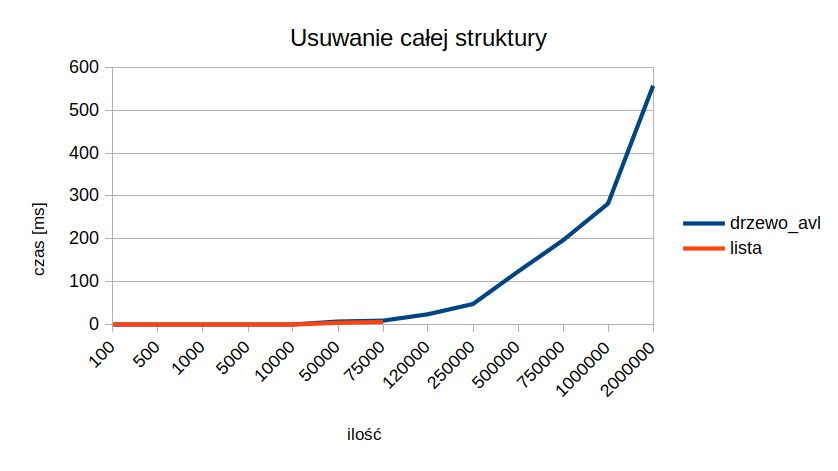
\includegraphics{remove_all.png}
			\end{figure}
			\subsubsection{Lista}
				Polega ono na rekurencyjny przejściu przez całą strukturę i usunięciu każdego elemntu. Przejście przez każdy element struktury zajmie dokłanie $n$ operacji, a to daje złożoność:
				\[
				O(n) = n	
				\]
			\subsubsection{Drzewo AVL}
				Algorytm usuwania całej struktury polega na przejżeniu wszystkich jej węzłów i ich usunięcie. Złożonośc tej operacj to:
				\[
				O(n) = n
				\]
			
\pagebreak
					
\section{Zastosowania}
	\subsection{Lista}
		\begin{itemize}
			\item Listy jako dynamiczne struktury danych mogą być stosowane do przechowywania danych, których ilość nie jest znana podczas uruchamiania programu.
			
			\item Lista zajmuje tylko tyle miejsca ile jest wymagane do przechowania danych, kosztem czasu dostępu do poszczegónych elemtów, dlatego można ją wykorzystać do przechowywania duzych ilośći danych, do których czas dostępu nie jest elemntem kluczowym
			
			\item Lista pozwala na przechowanie elementów o takich samych wartościach, co daje możliwośc tworzenia spisów posiadanych elemntów, których rozróżnianie nie jest potrzebne, np. policzenie mediany z ocen, bez wiedzy ile tych ocen faktycznie jest
		\end{itemize}
	\subsection{Drzewo AVL}
		\begin{itemize}
			\item Ze względu na to, że drzewo AVL jest strukturą dynamiczną, nie potrzeba określać jego wielkości/pojemności przy jego deklaracji. Pozwala to na przechowywanie w nim danych, których ilość nie jest znana przy uruchamianiu programu
			
			\item Opisywana struktura ze względu na swoją dynamiczność, zajmuje w pamięci tylko tyle miejsca ile jest potzebne na przechowanie danych, dlatego świetnie nadaje się do przechowywania dużych ilości informacji
			
			\item Binarna budowa drzewa pozwala na szybkie szukanie oraz stwierdzanie instnienia elementu o danym indeksie
			
			\item Możliwość przechowywania zmiennej ilości elementów i krótki czas dostępu, sprawia że drzewo AVL jest idealną strukturą do wykorzystania jako baza danych
		\end{itemize}
\pagebreak
\tableofcontents
\end{document}
